\chapter{Технологическая часть}

В данной части рассматривается выбор средств реализации, описывается структура классов программы и
приводится интерфейс программного обеспечения.


\section{Средства реализации}

В данной работе для реализации был выбран язык программирования C++~\cite{cpp}.
Выбор обусловлен тем, что средствами языка можно реализовать все алгоритмы структуры данных, выбранные в результате проектирования.

В качестве среды разработки был выбран CLion~\cite{clion} от компании JetBrains~\cite{jet}.
Эта среда обеспечивает удобство работы с проектами на C++, интеграцию с системой контроля версий, а также поддержку
инструментария для отладки и профилирования кода.

Для разработки графического интерфейса был выбран QtCreator~\cite{qtCreator}.
Для отображения сцены использована библиотека Qt~\cite{qt}. Для реализации векторных вычислений,
таких как операции над точками, векторами и матрицами, используется библиотека GLM~\cite{glm} (OpenGL Mathematics).

Для управления структурами данных, включая полигональные сетки рельефа, высотные карты, карты воды и отложений,
используются стандартные средства языка C++ и объектно-ориентированный подход.

\section{Структура программного обеспечения}

Для реализации программного обеспечения была выбрана объектно–ориентированная
парадигма программирования. В связи с этим были реализованы следующие классы:

\begin{enumerate}
    \item Camera -- класс, задающий камеру;
    \item Light -- класс, задающий источник света;
    \item Renderer -- Класс, отвечающий за визуализацию полигональной сетки;
    \item Mesh -- класс, реализующий полигональную сетку;
    \item Erosion -- класс, отвечающий за визуализацию водной эрозии;
    \item RenderWidget -- класс, содержащий генератор полигональной сетки, камеру, источник освещения и визуализатор эрозии.
\end{enumerate}

Структура программы в виде диаграммы классов изображена на рисунке~\ref{img:uml}.

\begin{figure}[H]
    \centering
    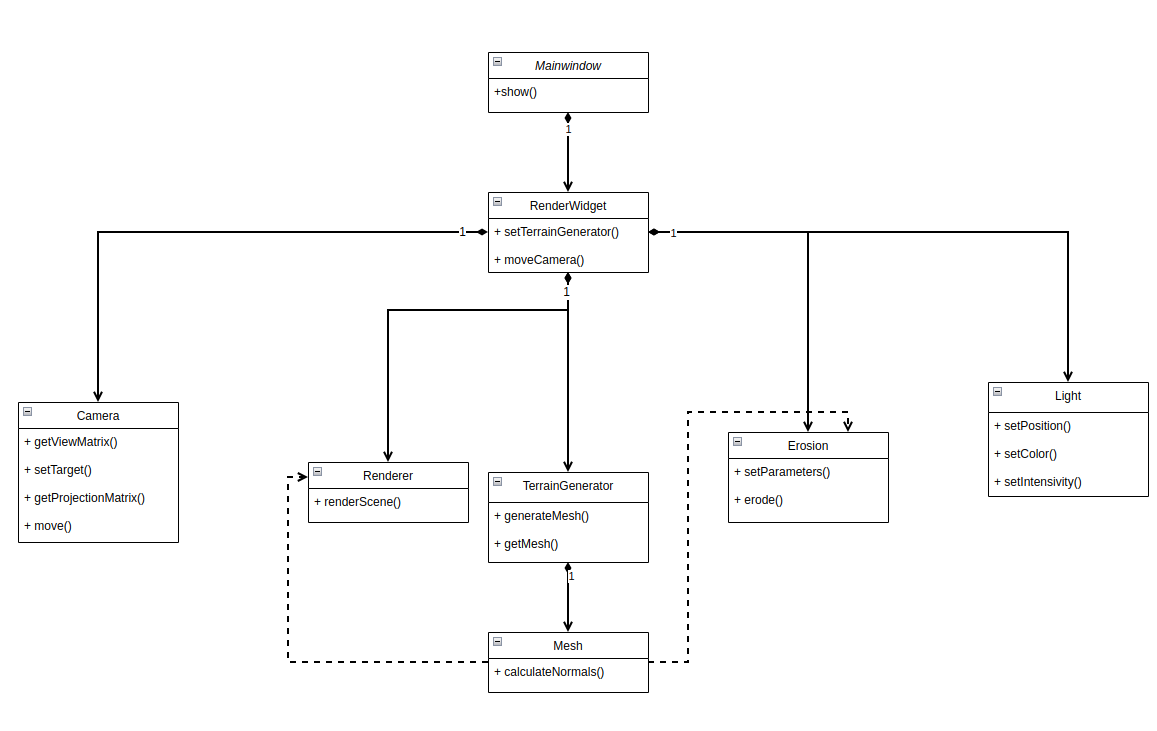
\includegraphics[scale=0.4]{images/uml}
    \caption{Диаграмма классов}
    \label{img:uml}
\end{figure}


\section{Реализация алгоритмов}

\subsection{Отрисовка треугольника}

На листинге~\ref{lst:rastr} приведена реализация алгоритма отрисовки треугольника с использованием Z буфера.

\begin{lstlisting}[style=cpp, label=lst:rastr, caption={Реализация функции renderTriangle}]
void Renderer::drawTriangleWithLocks(const Vertex& v0, const Vertex& v1, const Vertex& v2,
                                     const Light& light, const glm::mat4& mvpMatrix)
{
    for (int y = (int)minY; y <= (int)maxY; y++)
    {
        for (int x = (int)minX; x <= (int)maxX; x++)
        {
            glm::vec3 p((float)x + 0.5f, (float)y + 0.5f, 0.0f);
            float wA = edgeFunction(p1, p2, p);
            float wB = edgeFunction(p2, p0, p);
            float wC = edgeFunction(p0, p1, p);

            if (area > 0 && wA > 0 && wB > 0 && wC > 0 || area <= 0 && wA <= 0 && wB <= 0 && wC <= 0)
            {
                float lambda0 = wA / area;
                float lambda1 = wB / area;
                float lambda2 = wC / area;

                float invW = (lambda0 / w0) + (lambda1 / w1) + (lambda2 / w2);

                glm::vec3 fragPos = (pos0_over_w * lambda0 + pos1_over_w * lambda1 + pos2_over_w * lambda2) / invW;
                glm::vec3 fragNormal = (norm0_over_w * lambda0 + norm1_over_w * lambda1 + norm2_over_w * lambda2) /
                    invW;
                fragNormal = glm::normalize(fragNormal);

                float z = (p0.z * lambda0 + p1.z * lambda1 + p2.z * lambda2);

                int index = x + y * m_width;

                zBufferMutex.lock();
                float currentDepth = m_zBuffer[index];
                if (z < currentDepth)
                {
                    m_zBuffer[index] = z;
                    zBufferMutex.unlock();

                    glm::vec3 toLight = glm::normalize(lightPos - fragPos);
                    float lambert = glm::max(glm::dot(fragNormal, toLight), 0.0f);
                    glm::vec3 worldPos = lambda0 * v0.position + lambda1 * v1.position + lambda2 * v2.position;

                    glm::vec3 colorByHeight = getColorByHeight(-worldPos.y);
                    glm::vec3 fragColor = colorByHeight * lightColor * lambert;

                    frameBufferMutex.lock();
                    m_frameBuffer.setPixelColor(x, y, QColor(
                                                    static_cast<int>(fragColor.r * 255),
                                                    static_cast<int>(fragColor.g * 255),
                                                    static_cast<int>(fragColor.b * 255)
                                                ));

                    frameBufferMutex.unlock();
                }
                else
                    zBufferMutex.unlock();
            }
        }
    }
}
\end{lstlisting}

\subsection{Водная эрозия}

В листинге~\ref{lst:erosion} представлена реализация алгоритма водной эрозии.

\begin{lstlisting}[style=cpp, label=lst:erosion, caption={Реализация функции водной эрозии}]
void Erosion::applySingleIteration(TerrainGenerator& terrain)
{
    void Erosion::simulateDroplet(TerrainGenerator& terrain,
                              int startX, int startY,
                              int maxSteps,
                              float initialWater)
{
    int x = startX;
    int y = startY;

    float water    = initialWater;
    float sediment = 0.0f;

    for (int step = 0; step < maxSteps; ++step)
    {
        float currentHeight = terrain.at(x, y);

        float lowestHeight = currentHeight;
        int nx = x;
        int ny = y;

        for (int dy = -1; dy <= 1; ++dy)
        {
            for (int dx_ = -1; dx_ <= 1; ++dx_)
            {
                if (dx_ == 0 && dy == 0) continue;
                int xx = x + dx_;
                int yy = y + dy;
                if (!inRange(xx, yy)) continue;

                float neighH = terrain.at(xx, yy);
                if (neighH < lowestHeight) {
                    lowestHeight = neighH;
                    nx = xx;
                    ny = yy;
                }
            }
        }

        if (nx == x && ny == y)
        {

            float deposit = sediment * m_depositionRate;
            terrain.setAt(x, y, currentHeight + deposit);
            sediment -= deposit;

            break;
        }

        float slope = (currentHeight - lowestHeight);

        float erodeAmount = m_erosionRate * m_erosionStrength * slope;

        if (currentHeight > 0)
            erodeAmount = std::min(erodeAmount, currentHeight);

        if (erodeAmount > 0)
        {
            terrain.setAt(x, y, currentHeight - erodeAmount);
            sediment += erodeAmount;
        }

        float capacity = m_capacity * water;
        if (sediment > capacity)
        {
            float deposit = (sediment - capacity) * m_depositionRate;
            float newHeight = terrain.at(x,y) + deposit;
            terrain.setAt(x, y, newHeight);
            sediment -= deposit;
        }

        x = nx;
        y = ny;

        water -= (water * m_evaporation);
        if (water <= 0.00001f)
        {
            if (sediment > 0.0f)
            {
                float oldH = terrain.at(x,y);
                terrain.setAt(x, y, oldH + sediment);
                sediment = 0.0f;
            }
            break;
        }
    }
}
\end{lstlisting}

\section{Интерфейс программного обеспечения}

При запуске программы открывается окно, представленное на рисунке~\ref{img:win}.

\begin{figure}[H]
    \centering
    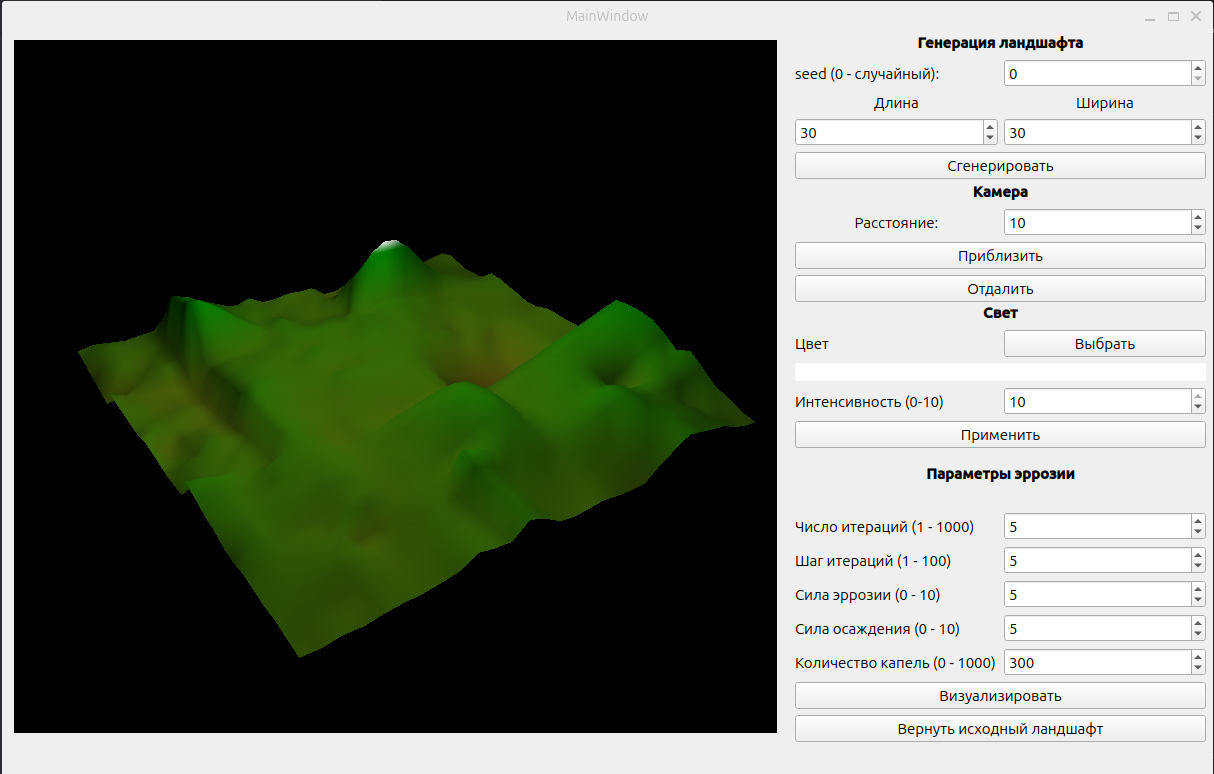
\includegraphics[scale=0.4]{images/wind}
    \caption{Окно программы}
    \label{img:win}
\end{figure}

Далее приведена информация о модулях интерфейса, с которыми пользователь может взаимодействовать.

\subsection*{Модуль изображения}

Пользователь может вращать камеру вокруг ландшафта при помощи клавиш A/D клавиатуры -- по горизонтали и W/S -- по вертикали.

\subsection*{Модуль генерации}

Пользователь может задать зерно генерации, а также длину и ширину итогового ландшафта.
Нажатие кнопки <<Сгенерировать>> создает ландшафт по введенному зерну генерации полученный ландшафт
визуализируется в модуле изображения.

\subsection*{Модуль камеры}

Нажатие кнопок <<Приблизить>> и <<Отдалить>> уменьшает и увеличивает расстояние до центра Ландшафта соответственно.

\subsection*{Модуль источника цвета}

Нажатие кнопки <<Выбрать>> открывает диалоговое окно с выбором цвета. После выбора цвета освещение сцены меняется.
Кнопка <<Применить>> изменяет значение интенсивности в соответствии с введенным значением.

\subsection*{Модуль эрозии}

Интерфейс позволяет задать следующие параметры эрозии:

\begin{itemize}
    \item число итераций;
    \item шаг итераций;
    \item сила эрозии;
    \item сила осаждения осадка;
    \item количество капель.
\end{itemize}

При нажатии на кнопку <<Визуализировать>> запускает процесс эрозии на введенное число итераций.
Изображение обновляется в соответствии с введенным значением шага.

На рисунке~\ref{img:doerr} представлено изображение рельефа до визуализации водной эрозии.

\begin{figure}[H]
    \centering
    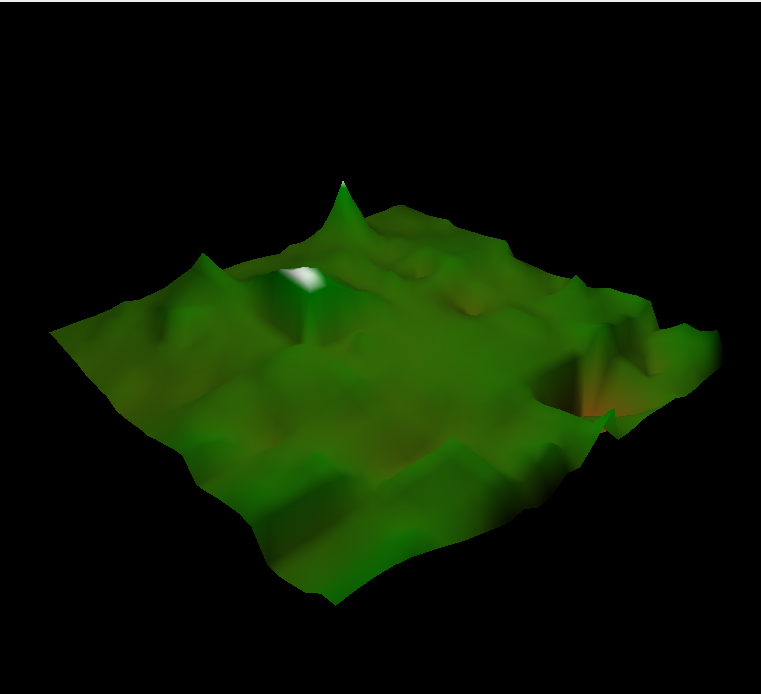
\includegraphics[scale=0.4]{images/doerr}
    \caption{Ландшафт до визуализации эрозии}
    \label{img:doerr}
\end{figure}

На рисунке~\ref{img:posterr} представлено изображение рельефа после 50 итераций водной эрозии.

\begin{figure}[H]
    \centering
    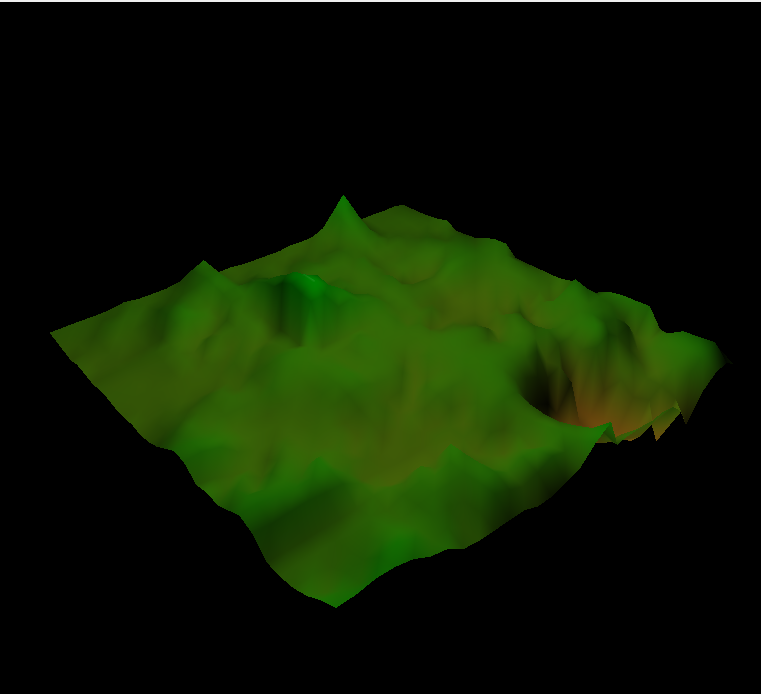
\includegraphics[scale=0.4]{images/posterr}
    \caption{Ландшафт после 50 итераций эрозии}
    \label{img:posterr}
\end{figure}

На рисунке~\ref{img:posterr2} представлено изображение рельефа после 100 итераций водной эрозии.

\begin{figure}[H]
    \centering
    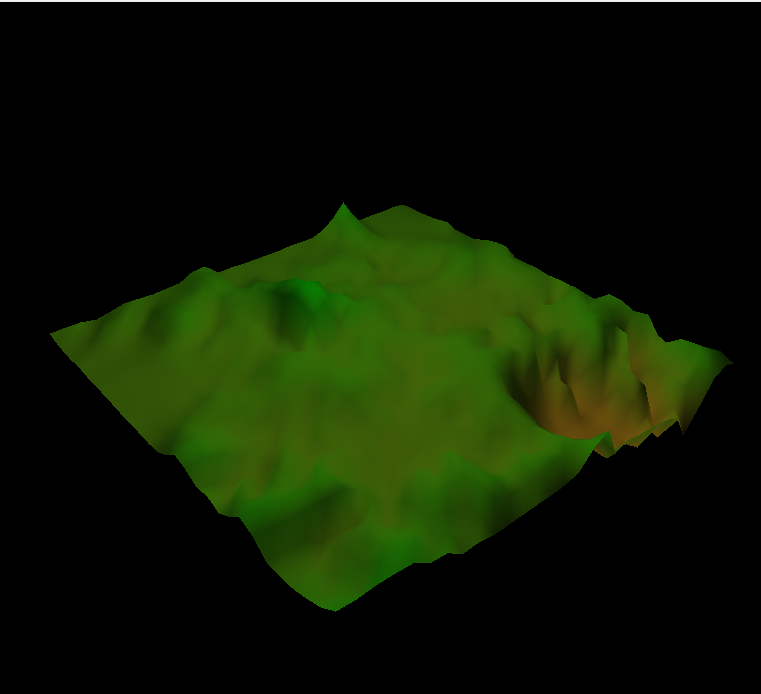
\includegraphics[scale=0.4]{images/posterr2}
    \caption{Ландшафт после 100 итераций эрозии}
    \label{img:posterr2}
\end{figure}

На рисунке~\ref{img:posterr3} представлено изображение рельефа после 200 итераций водной эрозии.

\begin{figure}[H]
    \centering
    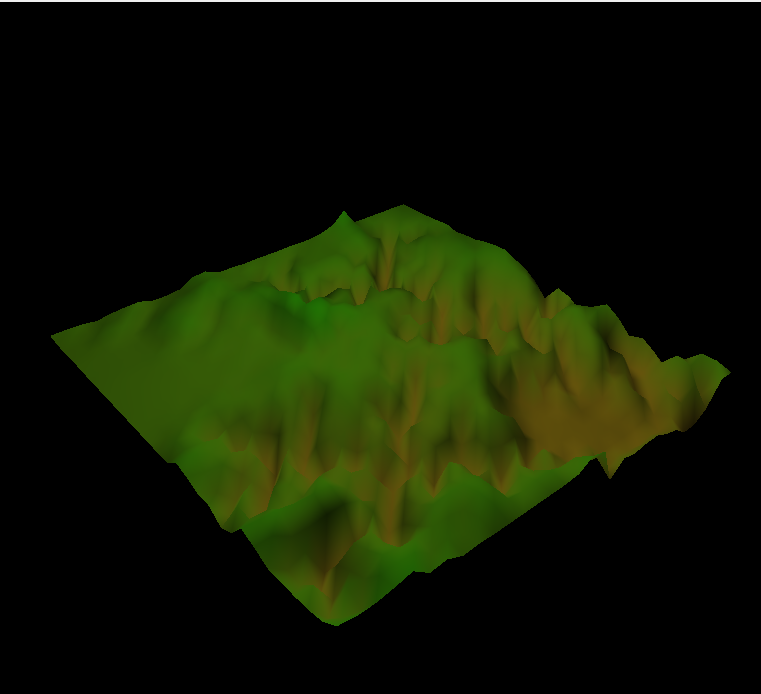
\includegraphics[scale=0.4]{images/posterr3}
    \caption{Ландшафт после 200 итераций эрозии}
    \label{img:posterr3}
\end{figure}

\section*{Вывод}

В этой части были приведены средства реализации. Также было реализовано ПО, выполняющее
визуализацию водной эрозии рельефа, пример работы которого представлен в этой части.

